\documentclass{beamer}

\usetheme{Warsaw}

\usepackage[utf8]{inputenc}
\usepackage[brazil]{babel}
\usepackage{listings}
\usepackage{graphicx}

\title[CV e fluxo de trabalho em projetos de software]{Controle de versão e fluxo de trabalho em projetos de
desenvolvimento de software}
\author{Antonio Terceiro}
\date{Novembro/2012}

\newcommand{\git}{\texttt{git}}
\newcommand{\cpr}{\texttt{cp -r}}
\newcommand{\rcs}{\texttt{rcs}}
\newcommand{\svn}{\texttt{svn}}
\newcommand{\cvs}{\texttt{CVS}}

\newcommand{\branch}{\emph{branch}}
\newcommand{\branches}{\emph{branches}}
\newcommand{\merge}{\emph{merge}}
\newcommand{\commit}{\emph{commit}}
\newcommand{\commits}{\emph{commits}}

\AtBeginSection[]
{
  \begin{frame}<beamer>{Roteiro}
    \tableofcontents[currentsection,hideallsubsections]
  \end{frame}
}

\lstset{%
  frame=shadowbox,
  rulesepcolor=\color{gray},
  numbers=left,
  basicstyle=\ttfamily\small,
  keywordstyle=\textbf,
  commentstyle=\color{gray}
}

\begin{document}
%%fakesection Material de capa
\begin{frame}[plain]
  \titlepage
\end{frame}

\begin{frame}
  \frametitle{Termos de uso}
  Este material pode ser usado segundo os termos da licença CreativeCommons
  Atribuição-Uso Não-Comercial-Compartilhamento pela mesma Licença 2.5 Brasil:

  \url{http://creativecommons.org/licenses/by-nc-sa/2.5/br/}

  Em resumo, é permitido:
  \begin{itemize}
    \item Copiar, distribuir, exibir e executar a obra
    \item Criar obras derivadas
  \end{itemize}
\end{frame}
\begin{frame}
  \frametitle{Termos de uso -- condições}
  Desde que:
  \begin{itemize}
    \item \structure{Atribuição.} Você deve dar crédito ao autor
      original, da forma especificada pelo Autor ou licenciante.
    \item \structure{Uso Não-Comercial.} Você não pode utilizar esta
      obra com finalidades comerciais.
    \item \structure{Compartilhamento pela mesma Licença.} Se você
      alterar, transformar, ou criar Outra obra com base nesta, você
      somente poderá distribuir a obra resultante sob Uma licença
      idêntica a esta.
  \end{itemize}

  Para cada novo uso ou distribuição, você deve deixar claro para outros os
  termos da licença desta obra.

  Qualquer uma destas condições podem ser renunciadas, desde que Você obtenha
  permissão do autor.
\end{frame}

\begin{frame}
  \frametitle{Resumo}

  Será apresentado um breve histórico dos sistemas de controle de
  versão livres, tanto do ponto de vista tecnológico quanto do modelo
  de fluxo de trabalho pressuposto pelos mesmos. Será dada ênfase em
  sistemas de controle de versão distribuído, em especial \git\
  (\url{http://git-scm.com/}), e como eles podem suportar diferentes
  \emph{workflows} em desenvolvimento de software.
\end{frame}

\begin{frame}
  \frametitle{Objetivos deste curso}
  \begin{itemize}
    \item Motivar para o uso de sistemas de controle de versão.
    \item Aprender conceitos básicos sobre a utilização de sistemas de
      controle de versão em geral.
    \item Introduzir o uso de \git, um sistema de controle de versão
      distribuído.
    \item Discutir possíveis \emph{workflows} em projetos de software, e
      como um sistema de controle de versão como \git\ pode suportá-los.
  \end{itemize}
\end{frame}

\begin{frame}{Roteiro}
  \tableofcontents[hideallsubsections]
\end{frame}

\section{Introdução}

\begin{frame}
  \frametitle{Motivação}
  \begin{itemize}
      \pause
    \item Todo software útil passará por mudanças.
      \pause
    \item As mudanças pelas quais o software passa precisam ser
      documentadas.
      \pause
    \item As várias mudanças específicas necessárias durante o ciclo de
      vida de um software devem poder ser:
      \pause
      \begin{itemize}
        \item separadas uma da outra
          \pause
        \item delimitadas no tempo e ordenadas
          \pause
        \item distribuídas por uma equipe
      \end{itemize}
  \end{itemize}
\end{frame}

\begin{frame}
  \frametitle{Sistemas de controle de versão}

  São sistemas que permitem armazenar conteúdo de forma que é possível:
  \pause

  \begin{itemize}
    \item Inspecionar o histórico de alterações a esse conteúdo;
      \pause
    \item Verificar o teor de uma alteração específica que pode ter
      acontecido num momento arbitrário do passado;
      \pause
    \item Gerenciar versões diferentes de conteúdo, e combiná-las de
      forma a gerar uma outra versão.
  \end{itemize}

  \pause
  No caso de desenvolvimento de software, esse conteúdo é o
  \structure{código-fonte}.

\end{frame}

\begin{frame}
  \frametitle{Por quê você deve usar controle de versão}
  
  \begin{itemize}
      \pause
    \item É possível determinar qual mudança introduziu um bug.
      \pause
    \item Você consegue ter acesso fácil a diferentes versões do software (produção,
      desenvolvimento etc)
      \pause
    \item É impossível desenvolver com equipes distribuídas sem usar
      controle de versão.
      \pause
    \item É possível identificar as mudanças exatas que foram necessárias
      para introduzir uma nova funcionalidade.
  \end{itemize}
\end{frame}

\section[Histórico]{Uma visão histórica dos sistemas de controle de versão}

\begin{frame}
  \frametitle{Uma visão histórica dos sistemas de controle de versão}

  \pause
  \begin{itemize}
    \item Objetivo: mostrar o histórico das ferramentas de controle de
      versão do ponto de vista do usuário, sem ressaltar diferenças nas
      implementações das ferramentas.
      \pause
    \item Reflete a minha experiência pessoal.
      \pause
    \item Provavelmente reflete a experiência pessoal de muitas outras
      pessoas que lidam com software livre há algum tempo.
  \end{itemize}
\end{frame}

\subsection{\cpr}

\begin{frame}{\cpr}
  \begin{itemize}
    \item Técnica mais primitiva -- e até intuitiva -- de controle de versão
    \item Bastante usada por quem tem costume de trocar documentos por
      e-mail.
      \begin{itemize}
        \item \texttt{projeto-v1.odt}, \texttt{projeto-v2.odt},
          \texttt{projeto-v3.odt} \ldots
      \end{itemize}
    \item em projetos de software, vai-se guardando cópias de diretórios
      inteiros para ``manter o histórico''.
  \end{itemize}
\end{frame}

\begin{frame}
  \frametitle{\cpr: Vantagens e desvantagens}
  \begin{itemize}
    \item Vantagens
      \begin{itemize}
        \item Não depende de nenhuma ferramenta
        \item Simples de fazer
      \end{itemize}
    \item Desvantagens
      \begin{itemize}
        \item Não mantém o histórico de alterações individuais
        \item Difícil de analisar
        \item Difícil de trabalhar em equipe
      \end{itemize}
  \end{itemize}
\end{frame}

\subsection{\rcs}

\begin{frame}
  \frametitle{\rcs}
  \begin{quote}
    The Revision Control System (RCS) manages multiple revisions of
    files. RCS automates the storing, retrieval, logging,
    identification, and merging of revisions. RCS is useful for text
    that is revised frequently, including source code, programs,
    documentation, graphics, papers, and form letters.
  \end{quote}

  \begin{itemize}
    \item \url{http://www.gnu.org/software/rcs/}
  \end{itemize}
\end{frame}

\begin{frame}
  \frametitle{\rcs, começando a usar ferramentas para controle de versão}
  \begin{itemize}
    \item Melhorias
      \begin{itemize}
        \item Já é possível trabalhar em equipe
      \end{itemize}

    \item Dificuldades restantes
      \begin{itemize}
        \item Desenvolvedores precisam ter acesso shell à mesma máquina.
        \item Ainda não é possível trabalhar em paralelo de verdade.
        \item Controle de versão é individualizado por arquivo.
      \end{itemize}
  \end{itemize}
\end{frame}

\begin{frame}
  \frametitle{\rcs: exemplo}
  \begin{figure}[h]
    \begin{center}
      \only<1>{\includegraphics[height=0.8\textheight]{figs/rcs-001.png}}%
      \only<2>{\includegraphics[height=0.8\textheight]{figs/rcs-002.png}}%
      \only<3>{\includegraphics[height=0.8\textheight]{figs/rcs-003.png}}%
      \only<4>{\includegraphics[height=0.8\textheight]{figs/rcs-004.png}}%
      \only<5>{\includegraphics[height=0.8\textheight]{figs/rcs-005.png}}%
    \end{center}
    \label{fig:rcs}
  \end{figure}
\end{frame}


\subsection{\cvs}

\begin{frame}
  \frametitle{\cvs}
  \begin{quote}
    CVS is a version control system, an important component of Source
    Configuration Management (SCM). Using it, you can record the history
    of sources files, and documents. It fills a similar role to the free
    software RCS, PRCS, and Aegis packages.
  \end{quote}

  \begin{itemize}
    \item Concurrent Versions System
    \item \url{http://www.nongnu.org/cvs/}
  \end{itemize}
\end{frame}

\begin{frame}
  \frametitle{\cvs, indo onde nenhum homem jamais esteve}
  \begin{itemize}
    \item Avanços
      \begin{itemize}
        \item Possível trabalhar em equipe em computadores
          diferentes.
        \item Possível para duas pessoas trabalharem no mesmo arquivo.
        \item Pode-se fazer referência ao estado de determinados
          arquivos num momento do tempo (tags)
      \end{itemize}
    \item Questões remanescentes
      \begin{itemize}
        \item Toda operação que envolve o histórico necessita que se
          esteja \emph{on-line}.
        \item Depende um repositório central.
        \item Controle de versão ainda é individualizado por arquivo.
      \end{itemize}
  \end{itemize}
\end{frame}

\begin{frame}
  \frametitle{\cvs: desenvolvimento distribuído}
  \begin{figure}[h]
    \begin{center}
      \only<1>{\includegraphics[height=0.8\textheight]{figs/cvs-001.png}}%
      \only<2>{\includegraphics[height=0.8\textheight]{figs/cvs-002.png}}%
      \only<3>{\includegraphics[height=0.8\textheight]{figs/cvs-003.png}}%
      \only<4>{\includegraphics[height=0.8\textheight]{figs/cvs-004.png}}%
    \end{center}
    \label{fig:cvs}
  \end{figure}
\end{frame}

\begin{frame}
  \frametitle{Interação de um desenvolvedor com repositório centralizado}
  \begin{figure}[h]
    \begin{center}
      \only<1>{\includegraphics[width=1\textwidth]{figs/centralized-interaction-001.png}}%
      \only<2>{\includegraphics[width=1\textwidth]{figs/centralized-interaction-002.png}}%
      \only<3>{\includegraphics[width=1\textwidth]{figs/centralized-interaction-003.png}}%
      \only<4>{\includegraphics[width=1\textwidth]{figs/centralized-interaction-004.png}}%
      \only<5>{\includegraphics[width=1\textwidth]{figs/centralized-interaction-005.png}}%
      \only<6>{\includegraphics[width=1\textwidth]{figs/centralized-interaction-006.png}}%
      \only<7>{\includegraphics[width=1\textwidth]{figs/centralized-interaction-007.png}}%
      \only<8>{\includegraphics[width=1\textwidth]{figs/centralized-interaction-008.png}}%
    \end{center}
    \label{fig:centralized-interaction}
  \end{figure}
\end{frame}

\subsection{\svn}

\begin{frame}
  \frametitle{\svn}
  \begin{itemize}
    \item \emph{``CVS done right''}
    \item \url{http://subversion.tigris.org/}
  \end{itemize}
\end{frame}

\begin{frame}
  \frametitle{\svn, um \cvs\ melhorzinho}
  \begin{itemize}
    \item Melhorou mesmo
      \begin{itemize}
        \item Commits atômicos: controle de versão da árvore inteira.
      \end{itemize}
    \item Manteve
      \begin{itemize}
        \item Ainda depende-se de estar \emph{on-line} para quase todas
          as operações.
        \item Ainda depende-se de um repositório centralizado.
      \end{itemize}
  \end{itemize}
\end{frame}

\begin{frame}
  \frametitle{\svn: exemplo}
  \begin{figure}[h]
    \begin{center}
      \only<1>{\includegraphics[height=0.8\textheight]{figs/svn-001.png}}%
      \only<2>{\includegraphics[height=0.8\textheight]{figs/svn-002.png}}%
      \only<3>{\includegraphics[height=0.8\textheight]{figs/svn-003.png}}%
      \only<4>{\includegraphics[height=0.8\textheight]{figs/svn-004.png}}%
    \end{center}
    \label{fig:svn}
  \end{figure}
\end{frame}


\subsection{Controle de versão distribuído}

\begin{frame}
  \frametitle{Problemas com controle de versão centralizado}
  \begin{itemize}
      \pause
    \item Necessidade de estar sempre conectado.
      \pause
    \item Desenvolvedor é forçado a resolver conflitos imediatamente.
      \pause
    \item Repositório central é um ponto central de falha.
      \pause
    \item Necessidade de conceder permissão de escrita explicitamente
      emperra a colaboração.
  \end{itemize}
\end{frame}

\begin{frame}
  \frametitle{Controle de versão Distribuído}

  Um sistema de controle de versão distribuído:

  \begin{itemize}
      \pause
    \item não depende de um repositório central.
      \pause
    \item permite que diferentes usuários evoluam em direções diferentes
      (\emph{branches}) a partir de um mesmo ponto comum.
      \pause
    \item oferece ferramentas para fazer \emph{merge} de diferentes
      \emph{branches} de volta ao \emph{branch} principal.
      \pause
    \item (entre outras características)
  \end{itemize}
\end{frame}

\begin{frame}
  \frametitle{Controle de versão distribuído}
  \begin{figure}[h]
    \begin{center}
      \only<1>{\includegraphics[height=0.8\textheight]{figs/distributed-vcs-001.png}}%
      \only<2>{\includegraphics[height=0.8\textheight]{figs/distributed-vcs-002.png}}%
      \only<3>{\includegraphics[height=0.8\textheight]{figs/distributed-vcs-003.png}}%
      \only<4>{\includegraphics[height=0.8\textheight]{figs/distributed-vcs-004.png}}%
    \end{center}
    \label{fig:distributed-vcs}
  \end{figure}
\end{frame}

\begin{frame}
  \frametitle{Resumindo a história}
  \begin{figure}[h]
    \begin{center}
      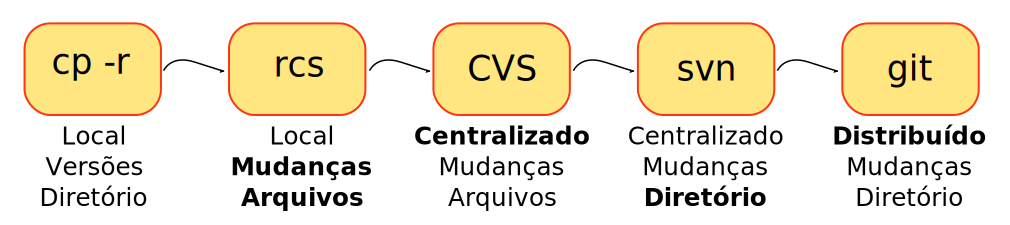
\includegraphics[width=1.0\textwidth]{figs/evolucao.png}
    \end{center}
    \caption{Evolução dos VCS, do ponto de vista do usuário}
    \label{fig:evolucao}
  \end{figure}
\end{frame}

\section[\git]{Controle de versão distribuído com \git}

\begin{frame}
  \frametitle{Sobre o \git}
  \begin{itemize}
    \item \url{http://git-scm.com/}
    \item Pacotes disponíveis para diversos sistemas operacionais.
    \item Principal interface: programa \git\ (linha de comando).
  \end{itemize}
\end{frame}

\subsection{Operação básica}

\begin{frame}
  \frametitle{Iniciando um repositório \git}
  \begin{itemize}
    \item \texttt{git init}\\
      Inicializa o repositório, criando um diretório \texttt{.git} na
      raiz do diretório atual.
      \pause

    \item \texttt{git add [ ARQ1 ARQ2 \ldots ]}\\
      Informa ao \git\ sobre arquivos que devem ser mantidos sob controle
      de versão.
      \pause

    \item \texttt{git commit}\\
      Confirma alterações nos arquivos mantidos sob controle de versão
      (ou que estão sendo incluídos).
  \end{itemize}
\end{frame}

\begin{frame}
  \frametitle{init, add, commit}
  \begin{figure}[h]
    \begin{center}
      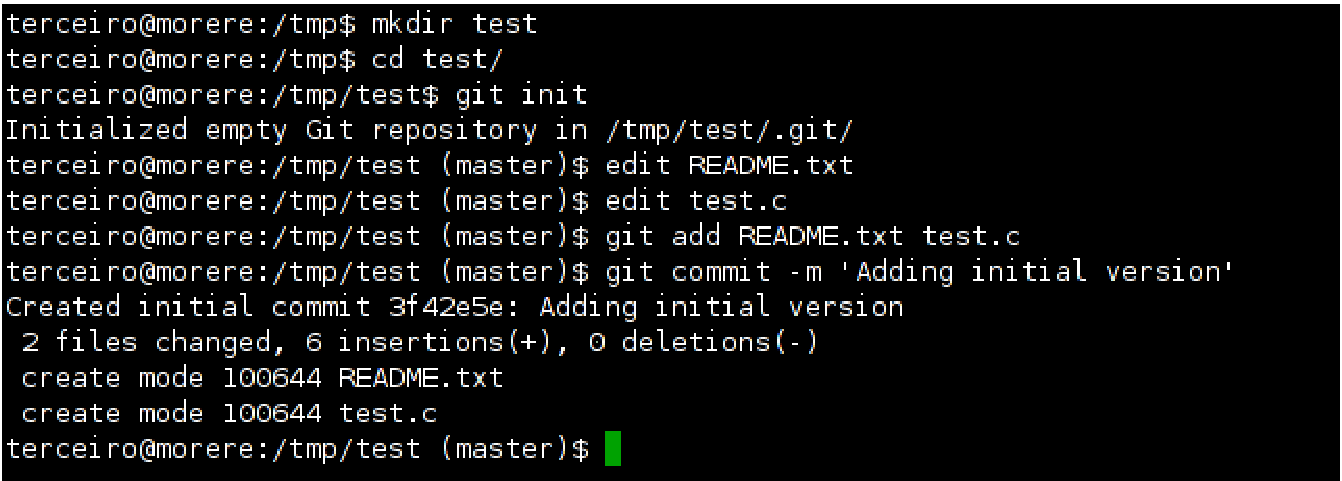
\includegraphics[width=0.85\textwidth]{figs/git-screenshot-init-add-commit.pdf}
    \end{center}
    \label{fig:git-init-add-commit}
  \end{figure}
\end{frame}

\begin{frame}
  \frametitle{Verificando trabalho realizado}
  \begin{itemize}

    \item \texttt{git diff}\\
      Lista as diferenças entre o conteúdo atual do diretório e o último
      \commit.
      \pause

    \item \texttt{git log}\\
      Lista todos os \commits\ realizados no \branch\ atual.
      \pause

    \item \texttt{git show [COMMIT]}\\
      Mostra o conteúdo de \texttt{COMMIT}, ou do topo do \branch\ atual
      se \texttt{COMMIT} é omitido.

  \end{itemize}
\end{frame}

\begin{frame}
  \frametitle{\texttt{git diff}}
  \begin{figure}[h]
    \begin{center}
      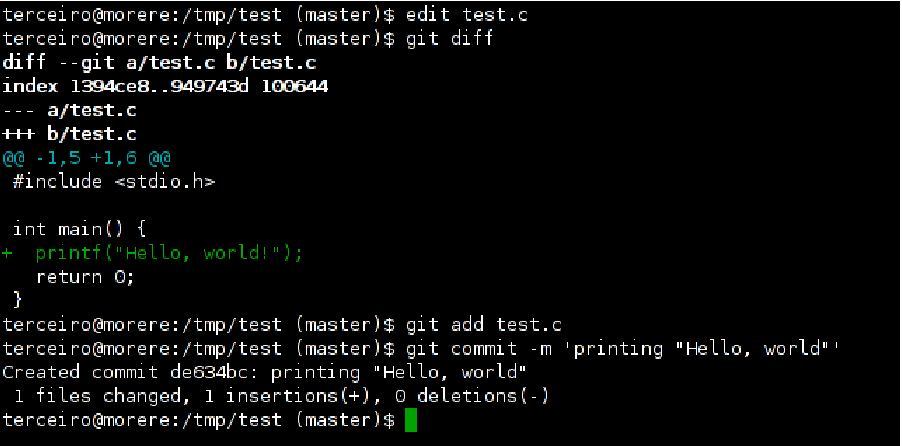
\includegraphics[width=0.85\textwidth]{figs/git-screenshot-diff.pdf}
    \end{center}
    \label{fig:git-diff}
  \end{figure}
\end{frame}

\begin{frame}
  \frametitle{\texttt{git log}}
  \begin{figure}[h]
    \begin{center}
      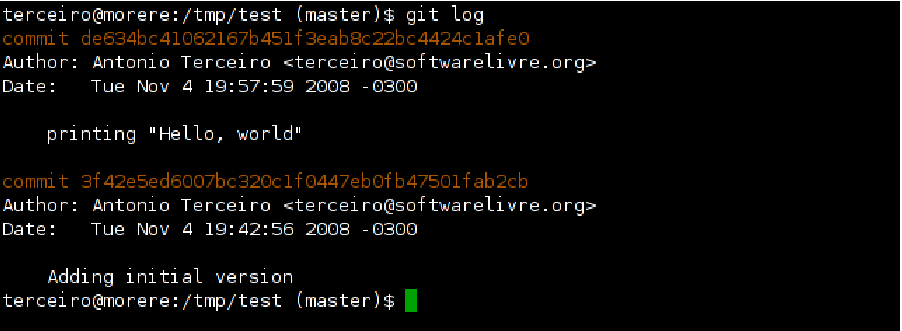
\includegraphics[width=0.85\textwidth]{figs/git-screenshot-log.pdf}
    \end{center}
    \label{fig:git-log}
  \end{figure}
\end{frame}

\begin{frame}
  \frametitle{\texttt{git show}}
  \begin{figure}[h]
    \begin{center}
      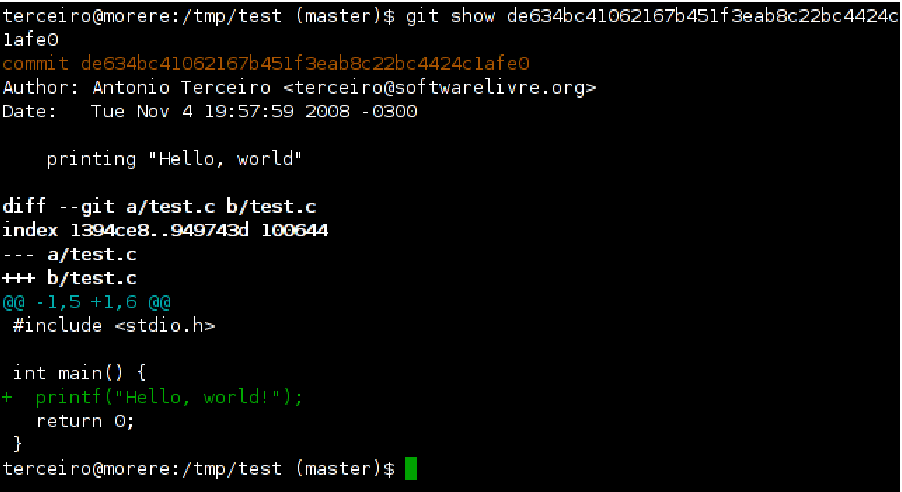
\includegraphics[width=0.85\textwidth]{figs/git-screenshot-show.pdf}
    \end{center}
    \label{fig:git-show}
  \end{figure}
\end{frame}

\begin{frame}
  \frametitle{Ferramentas gráficas}
  \begin{itemize}
    \item \texttt{gitk}.
    \item \texttt{giggle}.
    \item outras?
  \end{itemize}
\end{frame}

\subsection{Branching e merging}

\begin{frame}
  \frametitle{Branches}
  \begin{itemize}
    \item \texttt{git branch [NOVOBRANCH BRANCHANTIGO]}\\
      Cria um novo \branch\ com nome \texttt{NOVOBRANCH}, a partir do
      ponto onde está \texttt{BRANCHANTIGO}.
      \pause

    \item \texttt{git branch}\\
      Lista os branches existentes.
      \pause

    \item \texttt{git checkout [BRANCH]}\\
      Muda para o \branch\ \texttt{BRANCH}.
      \pause

    \item \texttt{git merge [BRANCH]}\\
      Combina no \branch\ atual as mudanças que estão no \branch\ 
      \texttt{BRANCH} e que não estão no \branch\ atual.
  \end{itemize}
\end{frame}

\begin{frame}
  \frametitle{branch, merge}
  \begin{figure}[h]
    \begin{center}
      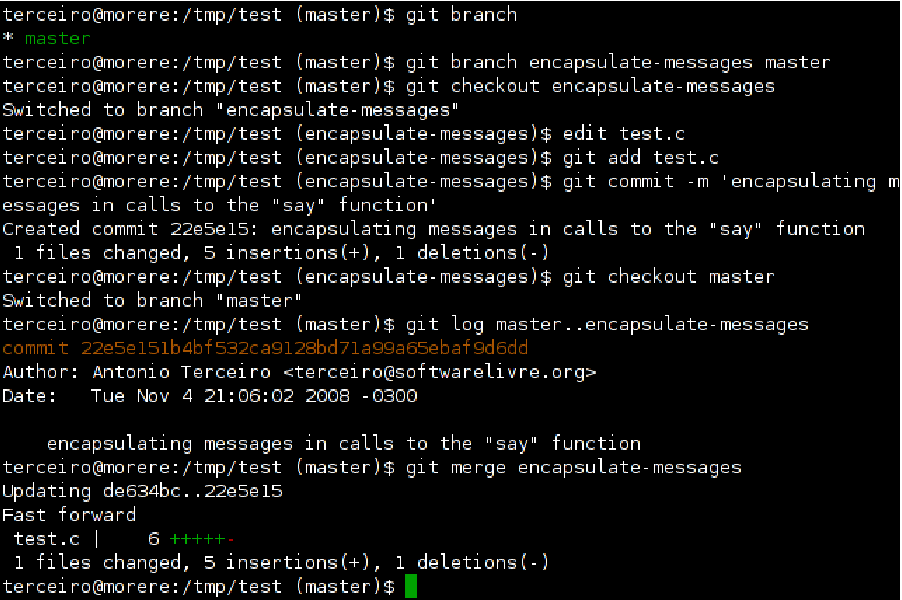
\includegraphics[width=0.85\textwidth]{figs/git-screenshot-branch-merge.pdf}
    \end{center}
    \label{fig:git-branch-merge-screenshot}
  \end{figure}
\end{frame}

\begin{frame}
  \frametitle{\emph{Branching} e \emph{merging}, graficamente}
  \begin{figure}[h]
    \begin{center}
      \only<1>{\includegraphics[height=0.8\textheight]{figs/git-branch-merge-001.png}}%
      \only<2>{\includegraphics[height=0.8\textheight]{figs/git-branch-merge-002.png}}%
      \only<3>{\includegraphics[height=0.8\textheight]{figs/git-branch-merge-003.png}}%
      \only<4>{\includegraphics[height=0.8\textheight]{figs/git-branch-merge-004.png}}%
      \only<5>{\includegraphics[height=0.8\textheight]{figs/git-branch-merge-005.png}}%
      \only<6>{\includegraphics[height=0.8\textheight]{figs/git-branch-merge-006.png}}%
      \only<7>{\includegraphics[height=0.8\textheight]{figs/git-branch-merge-007.png}}%
    \end{center}
    \label{fig:git-branch-merge}
  \end{figure}
\end{frame}

\begin{frame}
  \frametitle{Os dois tipos de merge}
  \begin{itemize}
    \item<1-> \merge ``tradicional'': quando os dois \branches\ já divergiram um o outro.
      \begin{itemize}
        \item Acabamos de ver um desses.
        \item Commit de \merge\ tem dois pais, o que faz o histórico
          deixar de ser linear.
      \end{itemize}
    \item<2-> \emph{Fast forward}: quando o \branch\ principal não tem
      atualizações em relação ao ponto a partir do qual o \branch\ do
      qual está se fazendo \merge\ foi criado.
      \begin{itemize}
        \item Não é necessária a criação de outro \commit.
        \item A ponta do \branch\ principal simplesmente é movida para a
          ponta do novo \branch .
        \item histórico de mantém linear.
      \end{itemize}
  \end{itemize}
\end{frame}

\begin{frame}
  \frametitle{\emph{Fast forward}}
  \begin{figure}[h]
    \begin{center}
      \only<1>{\includegraphics[height=0.8\textheight]{figs/git-fast-forward-001.png}}%
      \only<2>{\includegraphics[height=0.8\textheight]{figs/git-fast-forward-002.png}}%
      \only<3>{\includegraphics[height=0.8\textheight]{figs/git-fast-forward-003.png}}%
      \only<4>{\includegraphics[height=0.8\textheight]{figs/git-fast-forward-004.png}}%
      \only<5>{\includegraphics[height=0.8\textheight]{figs/git-fast-forward-005.png}}%
    \end{center}
    \label{fig:fast-forward}
  \end{figure}
\end{frame}

\begin{frame}
  \frametitle{\emph{Rebase}: reescrevendo o histórico}
  \begin{itemize}
    \item<1-> \texttt{git rebase BRANCH}\\
      Reaplica as mudanças realizadas no \branch\ atual a partir do
      ponto em que o \branch\ \texttt{BRANCH} foi criado em relação ao
      estado atual do \branch\ \texttt{BRANCH}, e move o branch atual
      para o último \commit\ resultante.
    \item<2-> Usado para linearizar o histórico.
    \item<3-> Não deve ser usado se o estado do branch atual já foi
      publicado.
  \end{itemize}
\end{frame}

\begin{frame}
  \frametitle{rebase, graficamente}
  \begin{figure}[h]
    \begin{center}
      \only<1>{\includegraphics[height=0.8\textheight]{figs/git-rebase-001.png}}%
      \only<2>{\includegraphics[height=0.8\textheight]{figs/git-rebase-002.png}}%
      \only<3>{\includegraphics[height=0.8\textheight]{figs/git-rebase-003.png}}%
      \only<4>{\includegraphics[height=0.8\textheight]{figs/git-rebase-004.png}}%
      \only<5>{\includegraphics[height=0.8\textheight]{figs/git-rebase-005.png}}%
      \only<6>{\includegraphics[height=0.8\textheight]{figs/git-rebase-006.png}}%
      \only<7>{\includegraphics[height=0.8\textheight]{figs/git-rebase-007.png}}%
    \end{center}
    \label{fig:rebase}
  \end{figure}
\end{frame}

\subsection[Repositórios remotos]{Lidando com repositórios remotos}

% clone
\begin{frame}
  \frametitle{Clonando um repositório}
  \begin{itemize}
    \item \texttt{git clone URL}\\
      Faz um clone local de um repositório público localizado em
      \texttt{URL}.
  \end{itemize}
\end{frame}

% remote
\begin{frame}
  \frametitle{Repositórios remotos em geral}

  \begin{itemize}
    \item \texttt{git remote add NAME URL}\\
      Associa o nome \texttt{NAME} ao repositório remoto publicado em
      \texttt{URL}
      \pause

    \item \texttt{git fetch NAME}\\
      Faz download dos objetos que estão no repositório remoto
      \texttt{NAME} mas que não estão no repositório local.
      \pause

    \item \texttt{git clone URL} é mais ou menos equivalente a:
      \begin{itemize}
        \item \texttt{git init}
        \item \texttt{git remote add origin URL}
        \item \texttt{git fetch origin}
        \item \texttt{git branch --track master origin/master}
      \end{itemize}
  \end{itemize}
\end{frame}

\begin{frame}
  \frametitle{Interagindo com repositórios remotos}
  \begin{itemize}
    \item \texttt{git fetch} de tempos em tempos
    \item \texttt{git merge origin/master} para aplicar as
      mudanças no \branch\ \texttt{master} remoto (\emph{``upstream''})
      ao \branch\ (\texttt{master}?) local.
      \pause

    \item \texttt{git pull} faz as duas coisas automaticamente:
      \begin{itemize}
        \item baixa os objetos presentes no repositório remoto de onde o
          \branch\ local atual foi derivado.
        \item Aplica as mudanças necessárias para fazer o \branch\ local
          atual igual ao \branch\ remoto original.
      \end{itemize}
      \pause

      É mais ou menos equivalente a:
      \begin{itemize}
        \item \texttt{git fetch origin}
        \item \texttt{git merge origin/master}
      \end{itemize}
  \end{itemize}
\end{frame}

% publicando um repositório
\begin{frame}
  \frametitle{Publicando um repositório}
  \pause
  \begin{itemize}
    \item \texttt{git remote add public [user@]server:/path/to/repo.git}
      \\
      Deve existir um repositório em \texttt{/path/to/repo.git} no
      servidor remoto \texttt{server}, e \texttt{user} deve ter acesso
      \emph{ssh} à máquina.
      \pause

    \item \texttt{git push public [master BRANCH1 BRANCH2 \ldots| --all]}
      \\
      Faz upload de todos os objetos presentes nos \branches\ locais
      \texttt{master BRANCH1 BRANCH2 \ldots} que também não estejam no
      repositório \texttt{public}, e atualiza esses \branches\ no
      repositório remoto para refletir seu estado no repositório local.
      \pause

    \item \texttt{git push} por \emph{default} empurra para o
      repositório ``\texttt{origin}''. 
  \end{itemize}
\end{frame}

\begin{frame}
  \frametitle{clone, pull}
  \begin{figure}[h]
    \begin{center}
      \includegraphics[width=0.85\textwidth]{figs/git-screenshot-clone-pull.pdf}
    \end{center}
    \label{fig:git-clone-pull}
  \end{figure}
\end{frame}

\begin{frame}
  \frametitle{push}
  \begin{figure}[h]
    \begin{center}
      \includegraphics[width=0.85\textwidth]{figs/git-screenshot-push.pdf}
    \end{center}
    \label{fig:git-push}
  \end{figure}
\end{frame}

\begin{frame}
  \frametitle{remote, fetch}
  \begin{figure}[h]
    \begin{center}
      \includegraphics[width=0.85\textwidth]{figs/git-screenshot-remote-fetch.pdf}
    \end{center}
    \label{fig:git-remote-fetch}
  \end{figure}
\end{frame}

% XXX \subsection[Outros]{Outros tópicos interessantes}
% TODO format-patch (?)
% TODO apply mailbox (?)
% TODO git-svn + comentar integração com outros VCS's
% bisect!
% comentar integração com outros VCS's

\section[Fluxo de Trabalho]{Fluxo de trabalho em projetos de desenvolvimento de software}

\begin{frame}
  \frametitle{Objetivos}
  \begin{itemize}
    \item Apresentar fluxos de trabalho comumente utilizados com o
      auxílio de sistemas de controle de versão.
    \item Identificar quais desses fluxos podem ser implementados com
      \begin{itemize}
        \item sistemas de controle de versão centralizados.
        \item sistemas de controle de versão distribuídos.
      \end{itemize}
    \item Discutir aplicabilidade desses fluxos a diferentes contextos,
      suas vantagens e desvantagens.
  \end{itemize}
\end{frame}

\begin{frame}
  \frametitle{3 diferentes fluxos de trabalho}
  \begin{itemize}
    \item Repositório central
    \item Gerente de Integração
    \item Ditador e Tenentes
  \end{itemize}
\end{frame}

\subsection{Repositório central}

\begin{frame}
  \frametitle{Repositório central}
  \begin{figure}[h]
    \begin{center}
      \only<1>{\includegraphics[height=0.8\textheight]{figs/central-repository-001.png}}%
      \only<2>{\includegraphics[height=0.8\textheight]{figs/central-repository-002.png}}%
      \only<3>{\includegraphics[height=0.8\textheight]{figs/central-repository-003.png}}%
      \only<4>{\includegraphics[height=0.8\textheight]{figs/central-repository-004.png}}%
      \only<5>{\includegraphics[height=0.8\textheight]{figs/central-repository-005.png}}%
      \only<6>{\includegraphics[height=0.8\textheight]{figs/central-repository-006.png}}%
    \end{center}
    \label{fig:centralized-repository}
  \end{figure}
\end{frame}

\begin{frame}
  \frametitle{Repositório central -- discussão}
  \begin{itemize}
    \item Aplicável com controle de versão centralizado e distribuído
    \item Vantagens
      \begin{itemize}
        \item<2-> Paralelismo.
        \item<3-> ``Simplicidade''.
      \end{itemize}
    \item Desvantagens
      \begin{itemize}
        \item<4-> Contribuições diretas dependem de permissão explícita de
          escrita no repositório.
        \item<5-> Sem um sistema de controle de versão distribuído, os
          contribuidores têm dificuldades em trabalhar em mais de uma
          funcionalidade/bug \emph{ao mesmo tempo}.
        \item <6->Repositório central é um ponto de falha.
      \end{itemize}
  \end{itemize}
\end{frame}

\subsection{Gerente de Integração}

\begin{frame}
  \frametitle{Gerente de Integração}
  \begin{figure}[h]
    \begin{center}
      \only<1>{\includegraphics[height=0.8\textheight]{figs/integration-manager-001.png}}%
      \only<2>{\includegraphics[height=0.8\textheight]{figs/integration-manager-002.png}}%
      \only<3>{\includegraphics[height=0.8\textheight]{figs/integration-manager-003.png}}%
    \end{center}
    \label{fig:integration-manager}
  \end{figure}
\end{frame}

\begin{frame}
  \frametitle{Gerente de Integração -- discussão}
  \begin{itemize}
    \item Difícil de aplicar sem controle de versão distribuído.
    \item Mais interação social entre os desenvolvedores.
    \item A depender do contexto, o gerente de integração pode ser uma
      máquina.
    \item Vantagens
      \begin{itemize}
        \item<2-> Atividade explícita de inspeção/revisão/teste.
        \item<3-> Maior controle sobre a base de código e sobre o design
          do software.
      \end{itemize}
    \item Desvantagens
      \begin{itemize}
        \item<4-> Gerente de Integração é um ponto de falha.
        \item<5-> Problemas de escala se o gerente de integração for
          humano.
        \item<6-> Pode ser difícil para equipes inexperientes.
      \end{itemize}
  \end{itemize}
\end{frame}

\subsection{Ditador e Tenentes}

\begin{frame}
  \frametitle{Ditador e Tenentes}
  \begin{figure}[h]
    \begin{center}
      \only<1>{\includegraphics[height=0.8\textheight]{figs/dictator-and-lieutenants-001.png}}%
      \only<2>{\includegraphics[height=0.8\textheight]{figs/dictator-and-lieutenants-002.png}}%
      \only<3>{\includegraphics[height=0.8\textheight]{figs/dictator-and-lieutenants-003.png}}%
      \only<4>{\includegraphics[height=0.8\textheight]{figs/dictator-and-lieutenants-004.png}}%
    \end{center}
    \label{fig:dictator-and-lieutenants}
  \end{figure}
\end{frame}

\begin{frame}
  \frametitle{Ditador e Tenentes -- discussão}
  \begin{itemize}
    \item Uma variação recursiva de ``Gerente de integração''.
    \item Praticamente impossível sem um sistema de controle de versão
      distribuído.
    \item Vantagens
      \begin{itemize}
        \item<2-> Melhor escalabilidade para projetos grandes.
        \item<3-> Menos pontos de falha
      \end{itemize}
    \item Desvantagens
      \begin{itemize}
        \item<4-> \ldots
      \end{itemize}
  \end{itemize}
\end{frame}

\section{Conclusões}

\begin{frame}
  \frametitle{Sistemas de controle de versão}
  \begin{itemize}
    \item É fundamental ter o histórico do desenvolvimento de um
      projeto.
    \item Uso conjunto com outras ferramentas pode fornecer ainda mais
      informação útil:
      \begin{itemize}
        \item integração com ferramentas de gestão de projetos (\emph{bug
          trackers})
        \item ferramentas de integração contínua
      \end{itemize}
  \end{itemize}
\end{frame}

\begin{frame}
  \frametitle{Workflows em projetos de software}
  Escolha depende de vários fatores
  \begin{itemize}
    \item<2-> Cultura e contexto da organização.
    \item<3-> Recursos.
    \item<4-> Demandas dos usuários.
    \item<5-> Demandas dos pares.
  \end{itemize}
\end{frame}

\begin{frame}
  \frametitle{Para saber mais: \git}
  \begin{itemize}
    \item \url{http://www.git-scm.org/}: manuais, tutoriais
    \item GitCasts: \url{http://www.gitcasts.com/}
    \item \texttt{git COMMMAND --help}\\
      ou\\
      \texttt{man git-COMMAND}
  \end{itemize}
\end{frame}

\begin{frame}
  \frametitle{Hospedagem de repositórios \git}
  \begin{itemize}
    \item Projetos de software livre:
      \begin{itemize}
        \item \url{http://gitorius.org/}
        \item \url{http://repo.or.cz/}
        \item \url{http://github.com/}
      \end{itemize}

    \item Projetos privados: \url{http://github.com/}
      \begin{itemize}
        \item planos por número de repositórios, número de
          colaboradores, espaço disponível etc.
      \end{itemize}
  \end{itemize}
\end{frame}

\begin{frame}
  \frametitle{Discussão}
  \begin{center}
    Contato: \texttt{terceiro@dcc.ufba.br}
  \end{center}
\end{frame}

\end{document}
